
This chapter describes the work done in each sprint. A sprint is one iteration
of the Scrum process (see section \ref{section:scrum} for more information about
Scrum). The duration of each sprint was two weeks. Every sprint was assigned
various tasks from the project backlog. Task IDs were assigned to task as they
were created. Each task was given a specific point value and assigned to one or
more team members. The point value is an estimation of the amount of work
(measured in man-hours) that is required to complete the task. The point value
can be also influenced by the importance of the task. If a task required more
time than planned and was not finished by the end of the sprint, it was assigned
a 'prolonged' status and moved to the next sprint.

For table layout reasons we used some name abbreviations for the names
of the members assigned to the task.

\begin{table}[ht!]
\begin{tabular}{ | c | l | }

\hline
\textbf{Abbreviation} & \textbf{Name} \\
\hline

 AN & \anders	\\
\hline
 AS & \asbjorn	\\
\hline
 B  & \bjornar	\\
\hline
 E  & \emanuele	\\
\hline
 JH & \johan	\\
\hline
 JN & \jonas	\\
\hline
 H  & \henrik	\\
\hline

\end{tabular}
\end{table}

\newpage

\section{Sprint 1}

Duration: 20/01 to 02/02
Points total: 89

The first sprint was dedicated to planning meetings and working hours
and studying about interested technologies. While some team members had some
experience with Arduino, none of us had any experience with Android application
development and social networks. Each member chose his own role in the project,
based on his own area of interest. The team did a lot of brainstorming in
order to identify possible product ideas to show the customer and produced a
small proof-of-concept application to show during the first meeting with the
customer, which was arranged for the beginning of the second week.

\begin{table}[ht!]
\begin{tabular}{ | r | l | c | c | r | }

\hline
\textbf{ID} & \textbf{Task} & \textbf{Points} & \textbf{Assigned to} & \textbf{Status} \\
\hline

 7 & Brainstorm ideas about the product		& 18 & Everyone		& done \\
\hline
 8 & Search for similar products			& 14 & Everyone		& done \\
\hline
 9 & Proof-of-concept application			& 12 & AN,B,E,JH	& done \\
\hline
11 & Read on OpenSocial						& 10 & E,H,JN		& done \\
\hline
13 & Read Facebook developers' pages		& 10  & E			& done\\
\hline
12 & Read on Arduino						& 8  & AN,AS,B,JH	& done \\
\hline
10 & Choose a development process			& 6  & Everyone		& done \\
\hline
 6 & Meet with the customer					& 4  & Everyone		& done \\
\hline
 2 & Plan group meetings					& 2  & Everyone		& done \\
\hline
 5 & Plan meetings with the customer		& 2  & Everyone		& done \\
\hline
 1 & Exchange contact information			& 1  & Everyone		& done \\
\hline
 4 & Setup mailing list						& 1  & JN			& done \\
\hline
 3 & Setup a Skype chat						& 1  & JH			& done \\
\hline

\end{tabular}
\end{table}

\newpage

\begin{figure}[h!]
\centering 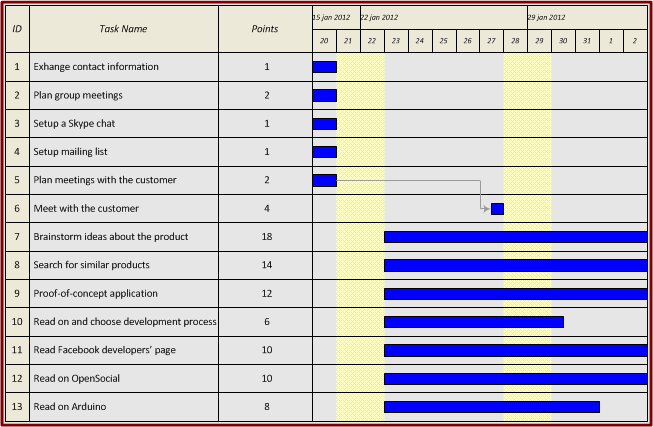
\includegraphics[scale=0.8]{img/sprints-gantt1.png}
\caption{Gantt diagram for the first sprint}
\label{fig:sprints-gantt1}
\end{figure}

\newpage

\section{Sprint 2}

Duration: 03/02 to 16/02
Points total: 96

The second iteration was focused on producing more prototypes of the product to
show the customer in order to receive the necessary feedback to identify
the product requirements and to begin designing the different parts of the
system, as well as acquiring the necessary knowledge and confidence with the
involved technologies. The team also worked on the preliminary version of the
report. The customer suggested that in order to show the re-usability
capabilities of the code, two more prototypes, considerably simpler than the
T-shirt prototype, could be produced for the project.

\begin{table}[ht!]
\begin{tabular}{ | r | l | c | c | r | }

\hline
\textbf{ID} & \textbf{Task} & \textbf{Points} & \textbf{Assigned to} &\textbf{Status} \\
\hline

 2 & Delivery of preliminary report				& 24 & Everyone		& done \\
\hline
 1 & Build a working prototype (week 1)			& 18 & Everyone		& done \\
\hline
 6 & Study Android app. develop.				& 18 & Everyone		& done \\
\hline
 7 & Study Facebook Android SDK					& 12 & E			& done \\
\hline
 3 & Build a working prototype (week 2)			& 8  & Everyone		& done \\
\hline
 4 & Bluetooth connection to Arduino			& 8  & AN,JH		& done \\
\hline
 5 & Connect to Facebook (FB SDK)				& 6  & E			& done \\
\hline
 8 & Setup ScrumDo								& 1  & AN,H			& done \\
\hline
 9 & Setup GIT repository						& 1  & JN			& done \\
\hline

\end{tabular}
\end{table}

\begin{figure}[h!]
\centering 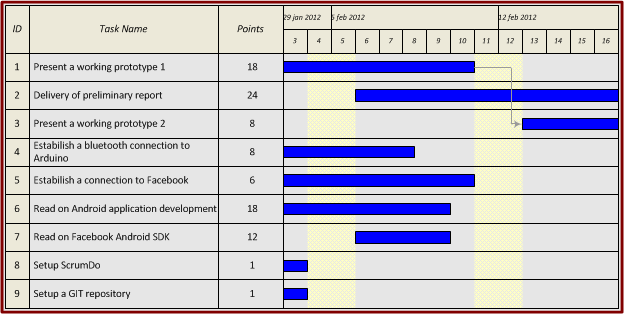
\includegraphics[scale=0.8]{img/sprints-gantt2.png}
\caption{Gantt diagram for the second sprint}
\label{fig:sprints-gantt2}
\end{figure}

\newpage

\section{Sprint 3}

Duration: 17/02 to 01/03
Points total: 108

This sprint was focused on proceeding with the design using the customer
feedback on the prototypes presented so far. An initial version of the
Communication library was also designed and coded. Design of the Social library
also began; various IPC solutions available in an Android system were taken into
consideration. During this sprint the system overall design started to take
shape, and the various parts of the system became more definite. The team
delivered a list of hardware needed to build the various T.U.I. prototypes.
The customer was happy with the team work so far and provided very valuable
feedback.

\begin{table}[ht!]
\begin{tabular}{ | r | l | c | c | r | }

\hline
\textbf{ID} & \textbf{Task} & \textbf{Points} & \textbf{Assigned to} & \textbf{Status} \\
\hline

 4 & Social library design (part 1/2)				& 20 & E		& done \\
\hline
 5 & Comm. library design (part 1/2)				& 20 & AN,JH	& done \\
\hline
 1 & Build a working prototype (week 1)				& 18 & Everyone & done \\
\hline
 6 & Comm. library coding (part 1/3)				& 16 & AN,JH	& done \\
\hline
 3 & Initial system design							& 14 & E,H		& done \\
\hline
 7 & Read on Android IPC mechanisms					& 12 & E		& done \\
\hline
 2 & Build a working prototype (week 2)				& 8 & Everyone	& done \\
\hline

\end{tabular}
\end{table}

\begin{figure}[h!]
\centering 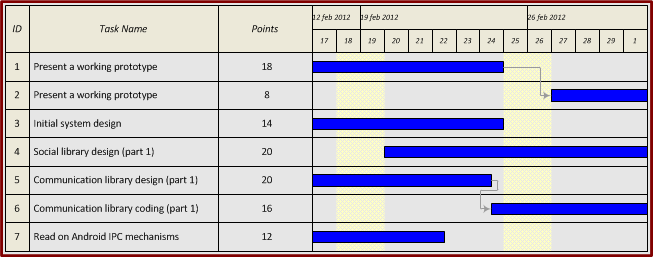
\includegraphics[scale=0.8]{img/sprints-gantt3.png}
\caption{Gantt diagram for the third sprint}
\label{fig:sprints-gantt3}
\end{figure}

\newpage

\section{Sprint 4}

Duration: 02/03 to 15/03
Points total: 112

This sprint was mainly aimed to the delivery of the mid-term report as well
as polishing of the Communication library. The system design proceeded as
planned while the design of the Social library couldn't be completed in time
due to some issues. The team had a hard time trying to find a satisfying
solution. These issues were presented to the customer who provided valuable
feedback that helped solve them.

\begin{table}[ht!]
\begin{tabular}{ | r | l | c | c | r | }

\hline
\textbf{ID} & \textbf{Task} & \textbf{Points} & \textbf{Assigned to} & \textbf{Status} \\
\hline

 1 & Work on the report					& 24 & Everyone & done \\
\hline
 2 & Build a working prototype			& 18 & Everyone & done \\
\hline
 3 & System design						& 18 & E 		& done \\
\hline
 7 & Comm. library coding (part 2/3)	& 16 & AN,JH	& done \\
\hline
 4 & Social libray design (part 2/2)	& 14 & E,H		& prolonged \\
\hline
 6 & Comm. library design (part 2/2)	& 12 & AN,JH	& done \\
\hline
 5 & Social library coding (part 1/3)	& 10 & E 		& done \\
\hline

\end{tabular}
\end{table}

\begin{figure}[h!]
\centering 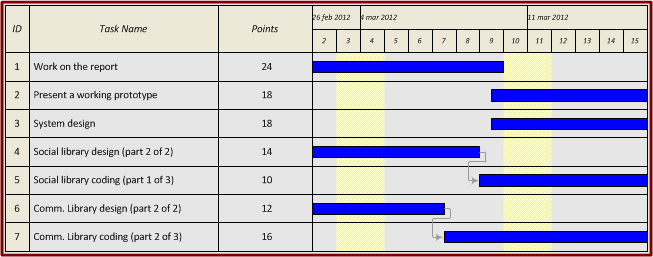
\includegraphics[scale=0.8]{img/sprints-gantt4.png}
\caption{Gantt diagram for the fourth sprint}
\label{fig:sprints-gantt4}
\end{figure}

\newpage

\section{Sprint 5}

Duration: 16/03 to 29/03
Points total: 128

During this sprint the team produced yet another prototype for the customer
and proceeded with the design and coding of the Social library. Coding of the
Communication library also continued, and an initial version was deployed by the
end of the sprint. The team also did some brainstorming and identified the other
two prototypes that were to be presented together with the T-shirt. Some
proof-of-concept applications for these prototypes were also made. This sprint
was a bit more intensive than the previous ones to cope with the fact that the
next sprint would have coincided with Easter vacation. The team still had not
received the hardware needed in order to begin building the T-shirt prototype.

\begin{table}[ht!]
\begin{tabular}{ | r | l | c |c | r | }

\hline
\textbf{ID} & \textbf{Task} & \textbf{Points} & \textbf{Assigned to} & \textbf{Status} \\
\hline

 2 & Social library design (part 2/2)			& 24 & E 		& completed \\
\hline
 4 & Comm. library coding (part 3/3)			& 22 & AN,JH	& done \\
\hline
 3 & Social library coding (part 2/3)			& 20 & E		& done \\
\hline
 1 & Build a working prototype					& 18 & Everyone	& done \\
\hline
 5 & Deploy the Comm. library					& 14 & JH		& done \\
\hline
 7 & Temp. prototype coding (part 1/2)			& 10 & B 		& done \\
\hline
 9 & Led prototype coding (part 1/2)			& 10 & AS 		& done \\
\hline
 6 & Temperature Prototype research				& 6  & B 		& done \\
\hline
 8 & Led prototype research						& 4  & AS 		& done \\
\hline

\end{tabular}
\end{table}

\begin{figure}[h!]
\centering 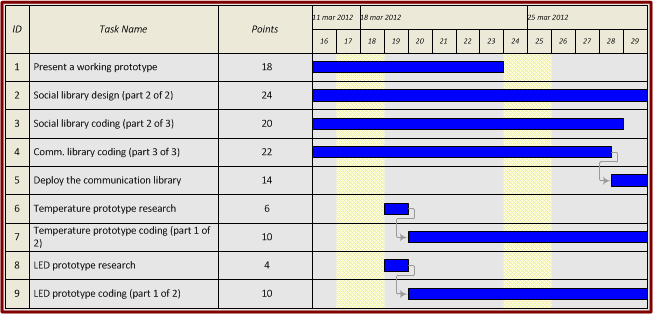
\includegraphics[scale=0.8]{img/sprints-gantt5.png}
\caption{Gantt diagram for the fifth sprint}
\label{fig:sprints-gantt5}
\end{figure}

\newpage

\section{Sprint 6}

Duration: 30/03 to 12/04
Points total: 50

As this sprint coincided with Easter vacation, little was planned for this
sprint except some early work on the report and some coding for the Social
library and the Temperature prototype. Some team members left the city, others
left the country. No meetings with the customer were arranged. The team had a
brief, sort of 'unplanned' meeting right before the vacation during which they
were told that the hardware had not yet been ordered.

\begin{table}[ht!]
\begin{tabular}{ | r | l | c | c | r | }

\hline
\textbf{ID} & \textbf{Task} & \textbf{Points} & \textbf{Assigned to} & \textbf{Status} \\
\hline

1 & Work on the report						& 18 & Everyone & done \\
\hline
2 & Social library coding (part 3/3)		& 18 & E		& done \\
\hline
3 & Temp. prototype coding (part 2/2)		& 14 & B		& done \\
\hline

\end{tabular}
\end{table}

\begin{figure}[h!]
\centering 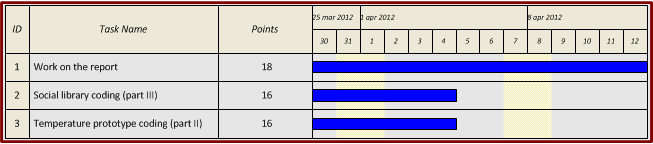
\includegraphics[scale=0.8]{img/sprints-gantt6.png}
\caption{Gantt diagram for the sixth sprint}
\label{fig:sprints-gantt6}
\end{figure}

\newpage

\section{Sprint 7}

Duration: 13/04 to 26/04
Points total: 130

Back from Easter vacation! Roughly one week after the group was back from
Easter vacation, the necessary hardware components needed for the product had
arrived. Also Mr. Babak, the customer, kindly provided a jacket that was to be
used for the final product. The various hardware devices were hooked up with the
Lilypad board and then tested individually, using a mockup application.

During this sprint the final product changed sightly from a T-shirt to a jacket.
The Lilypad board probably wasn't the best choice for a jacket product, in fact,
since the Arduino board could be hidden in a pocket, the team could have used
a smaller Arduino board, maybe with power connector and built-in battery
charger circuitry.

The Social library was finished, tested and an initial version deployed.
The Comm. lib started being thouroghly tested along with the prototypes.
Coding for the T-shirt application began. The Facebook and Twitter applications
started being converted from simple mockups to complete applications.

The team also worked on the delivery of the last supervised report.

\begin{table}[ht!]
\begin{tabular}{ | r | l | c | c | r | }

\hline
\textbf{ID} & \textbf{Task} & \textbf{Points} & \textbf{Assigned to} & \textbf{Status} \\
\hline

1 & Work on the report							& 22 & Everyone		& done \\
\hline
3 & T-Shirt app. coding (part 1/3)				& 22 & H			& done \\
\hline
2 & Build T-shirt prototype (part 1/3)			& 18 & AN,E,JH		& done \\
\hline
4 & Comm. library testing (part 1/2)			& 16 & AN,E,JH		& done \\
\hline
6 & Temp. prototype testing (part 1/2)			& 16 & B			& done \\
\hline
5 & Social library testing (part 1/2)			& 12 & E,H			& done \\
\hline
7 & Led prototype coding (part 2/2)				& 12 & AS			& done \\
\hline
8 & Facebook app. coding (part 1/2)				& 8  & E			& done \\
\hline
9 & Twitter application coding					& 4  & E			& done \\
\hline

\end{tabular}
\end{table}

\newpage

\section{Sprint 8}

Duration: 27/04 to 10/05
Points total: 168

As the deadline for the project began closing near, the sprints started to be
more intensive. During this sprint the team had some problems with the hardware
which slowed down the development of the prototype. The LCD screen that the team
was using stopped working probably due to wrong wiring. The team received a
spare one that was in the Lab a few days before the end of the sprint. As the
T-shirt T.U.I. changed into a jacket, the Lilypad board lost its main advantage
of being a sewable piece of hardware and the team started looking for alternative
Arduino boards, possibly with a battery socket and built-in recharge circuitry
which were missing in the Lilypad. Finally, a board with such features
(Arduino FIO) was chosen to substitute the Lilypad. A lot of testing involving
the Comm. lib was performed while building and testing the T-shirt prototype.
Testing was also performed for the other prototypes: Temperature and LED matrix.
The coding of the T-shirt and Facebook applications continued.
The T-shirt application couldn't be completed in time and was moved to the next
sprint. During one of the meetings, the customer liked an application that we
were using for testing the prototype functionality during the meeting's
demonstration and suggested the team to improve it and incorporate it in the
final product. This was rather unexpected as that application was only intented
for testing purposes. However the team added the client's request to their goals
for the next and final sprint.

\begin{table}[ht!]
\begin{tabular}{ | r | l | c | c | r | }

\hline
\textbf{ID} & \textbf{Task} & \textbf{Points} & \textbf{Assigned to} & \textbf{Status} \\
\hline

 1 & Build T-shirt prototype (part 2/3)			& 24 & AN,E,JH		& prolonged \\
\hline
 5 & T-shirt app. coding (part 2/3)				& 24 & H			& prolonged \\
\hline
 2 & Build a working prototype (week 1)			& 16 & Everyone		& done \\
\hline
 3 & Build a working prototype (week 2)			& 16 & Everyone		& done \\
\hline
 13 & Integration testing (part 1/2)			& 16 & Everyone		& done \\
\hline
 4 & Comm. library testing (part 2/2)			& 16 & AN,JH,E		& done \\
\hline
 7 & Work on the report							& 14 & Everyone		& done \\
\hline
 8 & Temp. prototype testing (part 2/2)			& 10 & B			& done \\
\hline
 10 & Facebook app. coding (part 2/2)			& 8  & E			& done \\
\hline
 12 & Facebook application testing				& 8  & E,H			& done \\
\hline
 6 & Social library testing (part 2/2)			& 6  & E			& done \\
\hline
 9 & Led prototype testing (part 1/2)			& 6  & AS			& done \\
\hline
 11 & Twitter application testing				& 4	 & E			& done \\
\hline

\end{tabular}
\end{table}

\newpage

\section{Final sprint}

Duration 11/05 to 25/05
Points total: 172

The final sprint, as in most software processes, was very intensive and aimed
to find as many errors as possible in the product.

The team continued in building the T-shirt T.U.I. prototype and testing
the oSNAP and T-shirt applications, and the system as a whole.
The LCD screen that the team was provided wasn't designed to work with the
voltage the Arduino FIO board was operating at: there were problems adjusting
the constrast. After considering various solutions to the problem, the team
opted to leave it like that since even if the contrast was off the text on the
display could still be read. During the first week the team held a presentation
of the product at a SINTEF office near the university. The presentation went
smoothly and the client seemed satisfied with the product. Since most of the
tasks for this sprint had to be completed before the presentation, the second
week was focused mostly on documentation work.


\begin{table}[ht!]
\begin{tabular}{ | r | l | c | c | r | }

\hline
\textbf{ID} & \textbf{Task} & \textbf{Points} & \textbf{Assigned to} & \textbf{Status} \\
\hline

 6 & Work on final report delivery				& 28 & Everyone	& done \\
\hline
 1 & Build T-shirt prototype (part 3/3)			& 24 & AN,E,JH	& completed \\
\hline
 5 & oSNAP application testing					& 24 & AN,E,JH	& done \\
\hline
 2 & T-Shirt app. coding (part 3/3)				& 18 & H		& completed \\
\hline
 4 & oSNAP application coding					& 18 & JH		& done \\
\hline
 9 & Integration testing (part 2/2)				& 16 & Everyone	& done \\
\hline
 3 & T-Shirt application testing 				& 14 & E,H		& done \\
\hline
 8 & System testing								& 12 & Everyone	& done \\
\hline
 7 & oSNAP WWW pages (market)					& 10 & JN		& done \\
\hline
10 & Led prototype testing (part 2/2)			& 8  & AS		& done \\
\hline
11 & Prepare a presentation of our project or products to SINTEF & 8  & Everyone       & done \\
\hline
12 & Present to SINTEF & 1  & Everyone       & done \\
\hline

\end{tabular}
\end{table}

\newpage

\begin{figure}[h!]
\centering 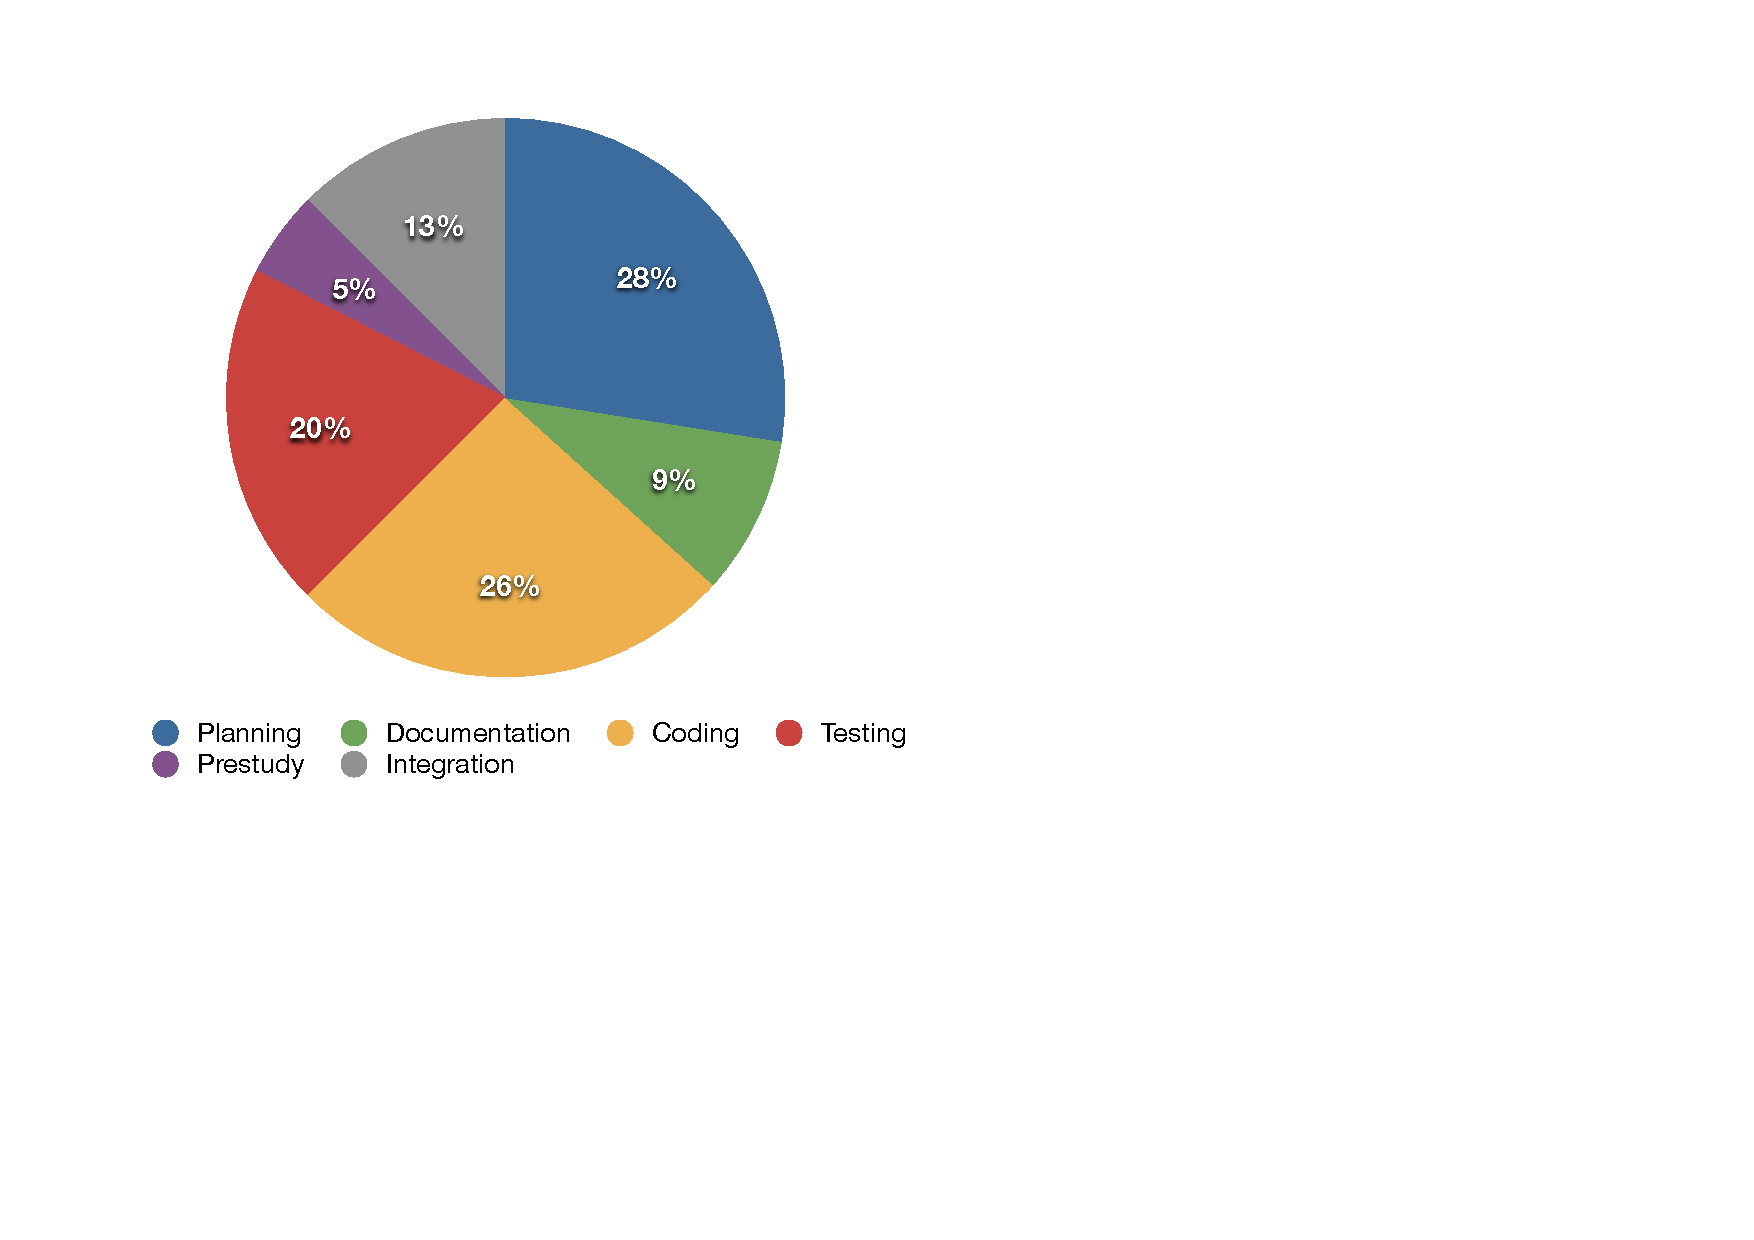
\includegraphics[scale=0.8]{img/pie_chart.pdf}
\caption{Story points breakdown}
\label{fig:sprints-points}
\end{figure}

\todo{
	update?
}
